\section{Linear Reward Penalty}
\subsection{Principe}

\begin{frame}{Principe}
\begin{itemize}
    \item Repose sur un \textbf{principe de récompense} lors d'une action positive.
    \item \textbf{Pénalise} les mauvaises actions.\\~\
    \item On obtient un \textbf{vecteur stochastique de stratégies} pour chaque carte et joueurs qui \textbf{se met à jour lors d'un gain ou d'une perte}.
\end{itemize}
\end{frame}

\begin{frame}{Mise à jour des stratégies des joueurs}
    \begin{block}{Règle de Mise à jour}
    \fontsize{8pt}{15pt}
    $q_{i,s}(t+1)=\left\{
    \begin{array}{ll}
        q_{i,s}(t)+b*U_{t}*(1-q_{i,s}(t))-\beta*q_{i,s}(t)* (1-U_{t}) & \mbox{Si } s=s_i(t) \\
         q_{i,s}(t)-b*U_{t}*q_{i,s}(t)+\beta*((k-1)^{-1}- q_{i,s}(t))*(1-U_{t}) & \mbox{Si } s\neq s_i(t)
    \end{array}
\right.$
    \end{block}
    
    \begin{exampleblock}{Variables et constantes}
    \begin{description}
    
    \item[b] : paramètre d'apprentissage tq $b \in [0,1]$ et $b\leq \frac{1}{U_{max}}$.
    \item[$\beta$] : paramètre d'apprentissage tq $\beta \in [0,1]$
    \item[k] : nombre total des actions.
    \item[$q_{i,s}(t)$] : probabilité que le joueur i joue la stratégie s à l'étape t.
    \item[$U_t$] : fonction d'utilité. %$U_t = \frac{Gain}{GainMax} =  \frac{Gain}{5}$
    
    \end{description}
    \end{exampleblock}
    
\end{frame}

\begin{frame}{Mise à jour des stratégies des joueurs}
    \begin{block}{Règle de Mise à jour}
    \fontsize{8pt}{15pt}
    $q_{i,s}(t+1)=\left\{
    \begin{array}{ll}
        q_{i,s}(t)+b*U_{t}*(1-q_{i,s}(t))-\beta*q_{i,s}(t)* (1-U_{t}) & \mbox{Si } s=s_i(t) \\
         q_{i,s}(t)-b*U_{t}*q_{i,s}(t)+\beta*((k-1)^{-1}- q_{i,s}(t))*(1-U_{t}) & \mbox{Si } s\neq s_i(t)
    \end{array}
\right.$
    \end{block}
    
    \begin{exampleblock}{Décision du choix des règles}
    
    $\left\{\begin{array}{ll}
    Linear\quad Reward\quad Penalty & \mbox{Si } b = \beta  \\
    Linear\quad Reward\quad Inaction & \mbox{Si } \beta = 0 \\
    Linear\quad Reward\quad \varepsilon-Penalty & \mbox{Si } b >> \beta 
    \end{array} 
    \right.$
    
    \end{exampleblock}
    
\end{frame}

\subsection{Application}

\begin{frame}{Etude de courbes}
    \begin{columns}
        \begin{column}{0.5 \textwidth}
        \begin{small}
        \hspace{-0.24 cm} Probabilité qu'\textcolor{red}{Alice} relance de 4 \\  Probabilité que \textcolor{blue}{Bob} suive\\
        \end{small}
        \centering
            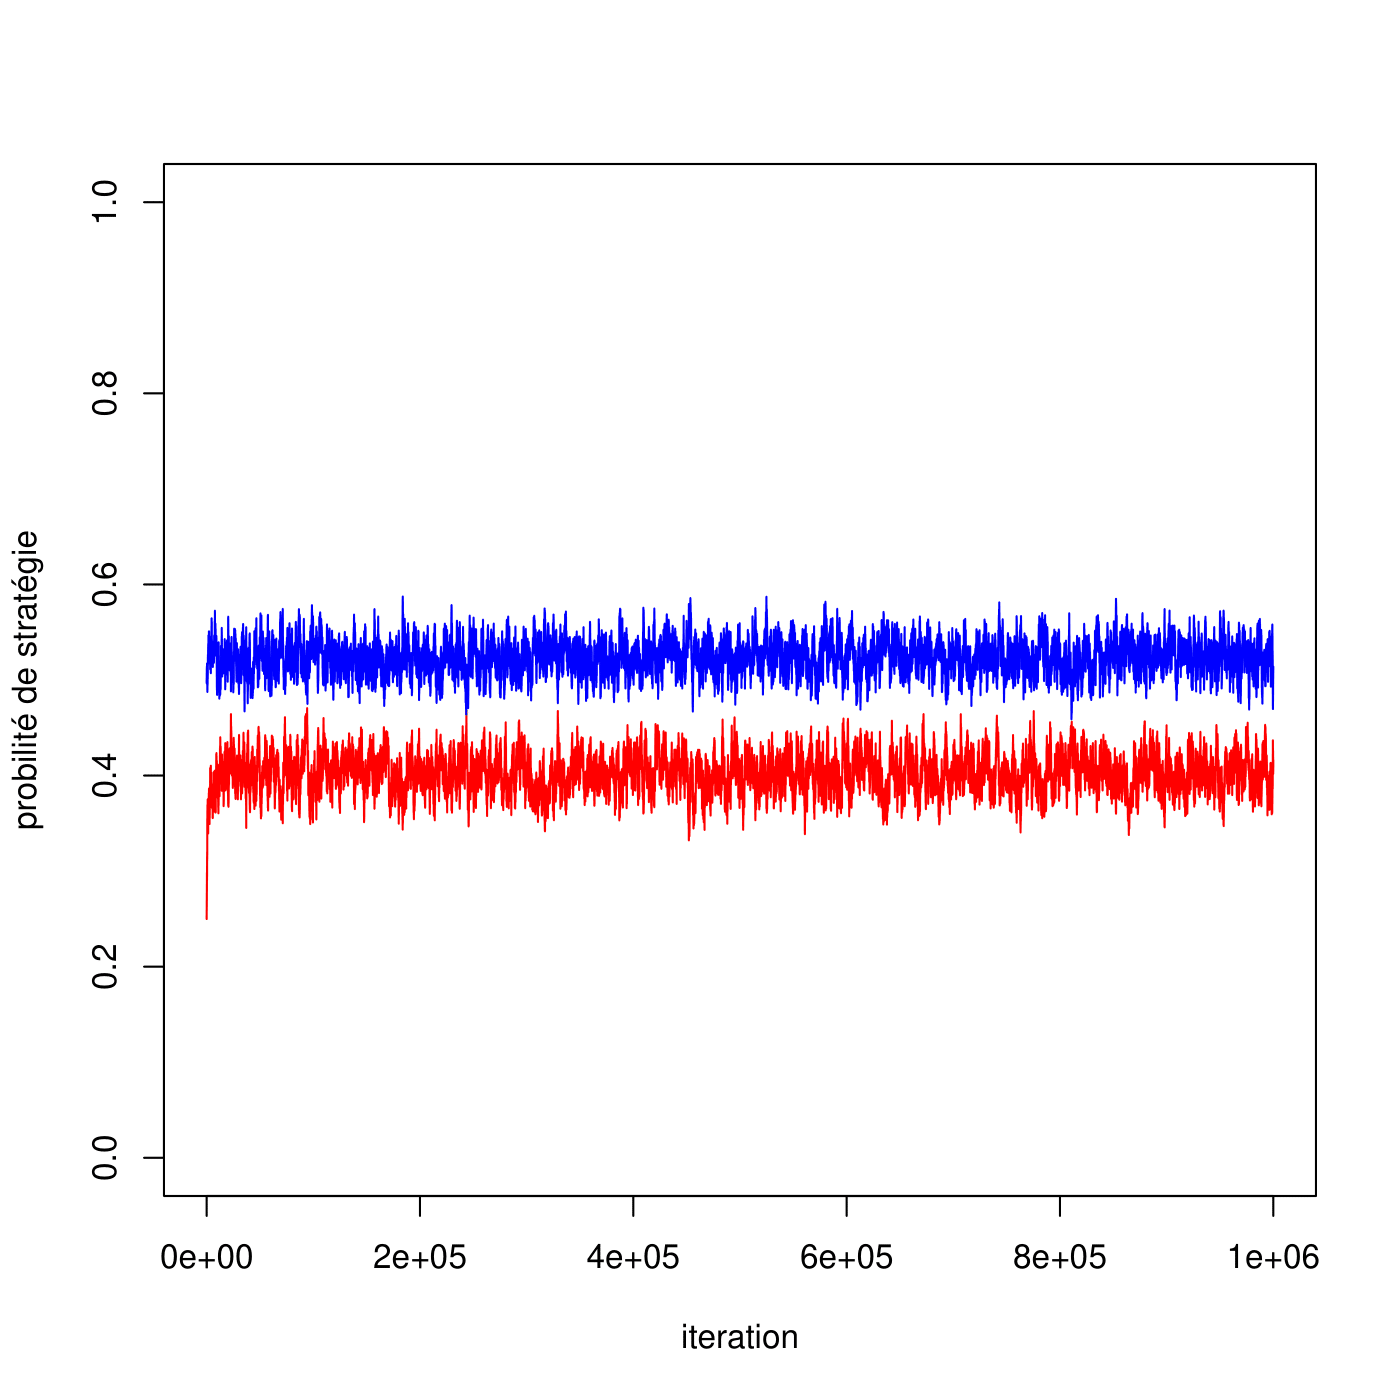
\includegraphics[width =\textwidth]{Images/Courbes/lrp-1.png}
       
    
        \end{column}
       
        \begin{column}{0.5 \textwidth}
         \begin{small}
          \hspace{-0.24 cm} Gain total d'\textcolor{red}{Alice} et de \textcolor{blue}{Bob} 
          \end{small}
        \centering
            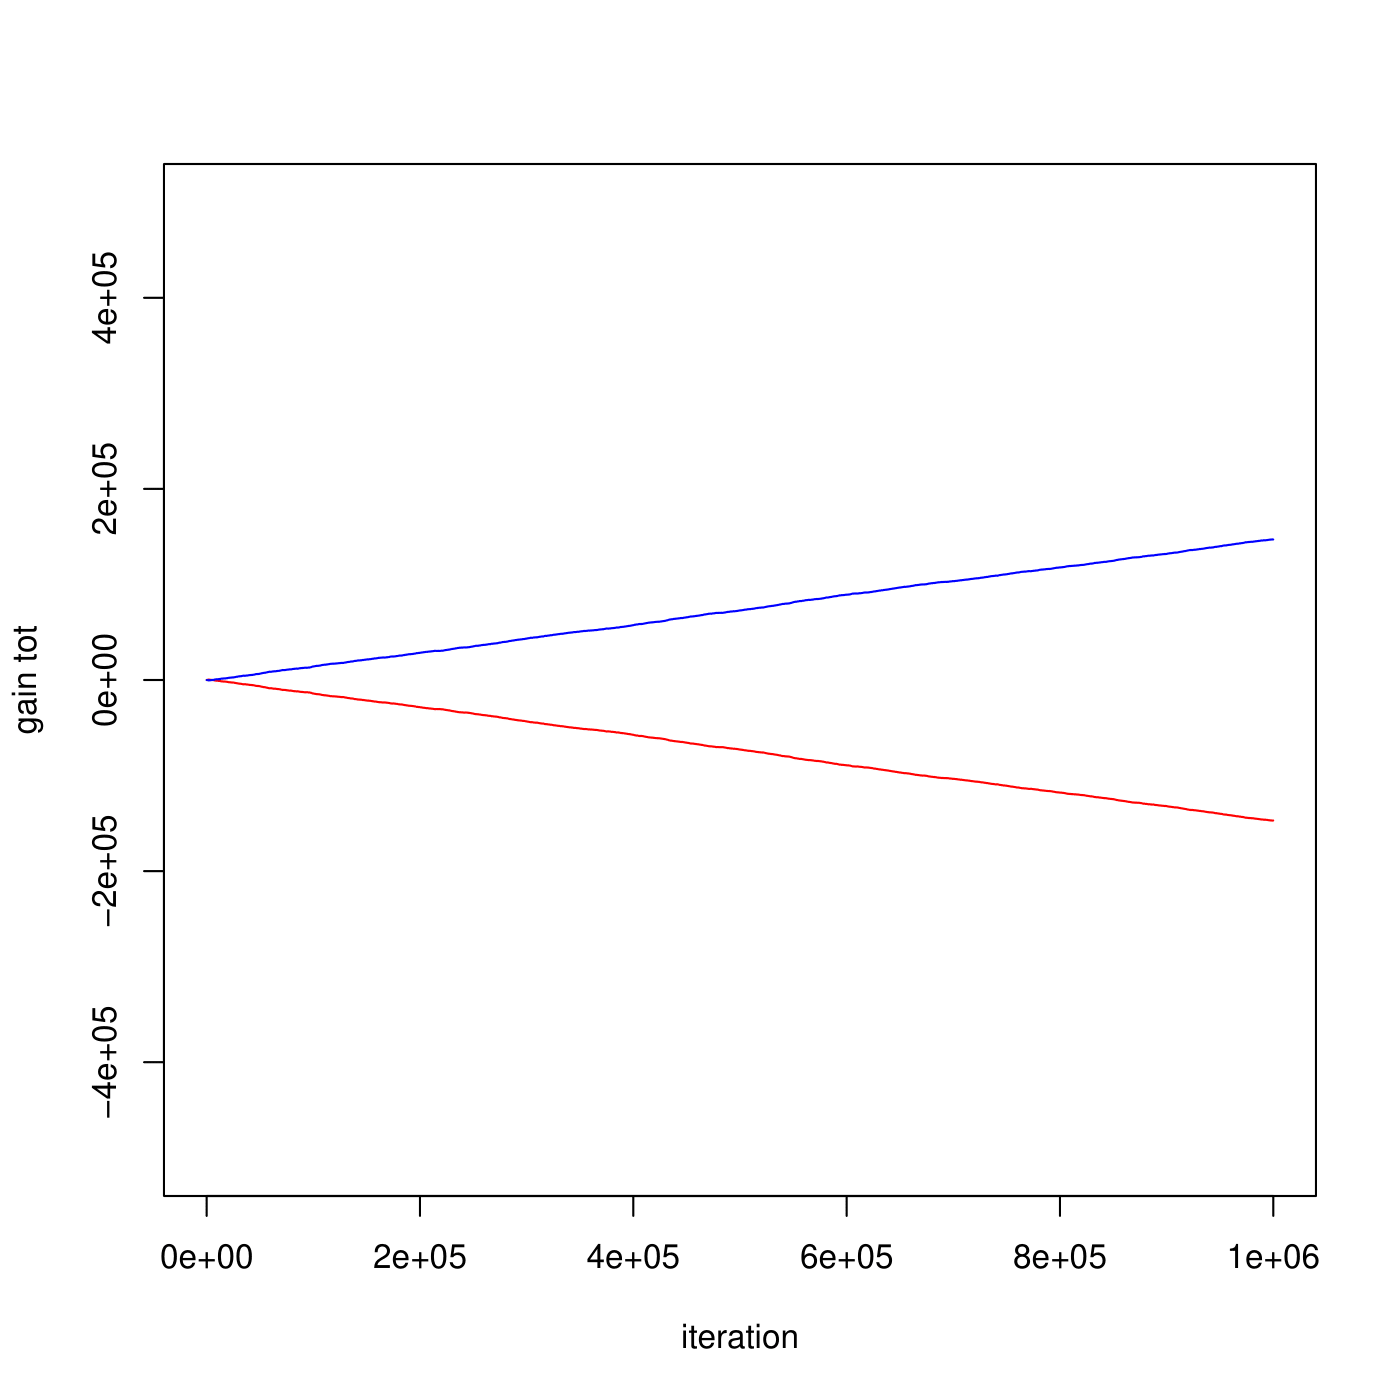
\includegraphics[width =\textwidth]{Images/Courbes/lrp-2.png}
       \end{column}
        \end{columns}



    
\end{frame}